\section{Quality Assurance}
\label{sec:quality_assurance}

\paragraph{Primary textual contributors:}
\mbox{}\\\emph{Oleksandr Huba}

Software development is more about people, rather than about technologies. That is why there is always a possibility of changing requirements from the business side or the risk of some bug occurring (e.g., because of a mistake from a developer), which can damage the performance of the product. There are a lot of other examples of obstacles which can appear during the development, but they all have the same effect – they negatively affect the quality of the product.

Quality is a crucial aspect of every software product. Good quality allows the business side to present their product in the best light and successfully compete in the market, because the user always chooses what is best. Quality cannot be neglected because it will make the product stand out negatively from the rest. So, if the development team tries to save money or time and thus does not pay enough attention to the level of quality, there will definitely come another, higher quality product to market, sooner rather than later.

In order to find a balance between all factors during the development process, quality assurance techniques shall be used. Our team applied different methods for assuring the quality of the SWTcamper application. These methods helped us to develop a reliable product and to satisfy customer and client requirements as much as we could. These quality assurance techniques are listed below.

\subsection{INVEST criteria}
During the project-blastoff our team created a list of user stories regarding desired functionality for every perspective. For this we used the project brief, which concisely and clearly describes requirements issued by client and customer.

This process was crucial for us, because we planned which functionality shall be implemented during each sprint based on these user stories. We also derived concrete tasks from the user stories. That is why we used the INVEST criteria during the creation of our user stories:

Our user stories are \emph{independent} from each other. This means that it allowed team members to implement a valuable working increment for the product without focusing on or waiting for completion of another user story.

Our user stories are \emph{negotiable}. Since our team didn’t have enough experience, we sometimes had to rewrite user stories, or change acceptance criteria in order to achieve the desired results by the end of each sprint. We tried to create each user story in such a way that there is enough room for further discussion between the development team and customer/client. This is important, because it gives customer and client the opportunity to participate in the development process and to ensure that their requirements are understood correctly.

The next important criterion for user stories is: each user story shall be \emph{valuable}. At the end of each sprint, we had to present a new feature to customer and client. Without this criterion, it would have been way harder to determine whether the work planned for and done during a sprint was even worth doing. We tried to avoid a situation where the business side is presented with the current increment and asks: “What benefit does that even bring me?”. Thus, we tried to implement high-priority user stories first, in order to provide the business side with the main functionalities as fast as possible.

During the first two sprints we had trouble estimating the size of user stories. However, later, we started to duly appreciate the criterion of a user story being \emph{estimable}. We defined 3 types of sizes and decided to apply them to every user story we had written. Size L is the biggest one, it corresponds to quite a big volume of work. User stories with size L took around 7 days of work for 2 developers. Next, there was size M, which corresponds to 5 days of work for 1 developer. And finally, user stories with size S took approximately 1-2 days for 1 developer. Estimation played a huge role in planning the sprint goals, because using our custom sizes, we could determine whether we will make it in time or not.

Our team aimed to create \emph{small} user stories in order to be able to fit a few features into a sprint goal instead of one gigantic one. We understood that it is more convenient to work with small user stories because it is easier for the whole team to derive concrete tasks and to keep track of the development progress.

Last but not least, user stories shall be \emph{testable}. In order to fulfill this characteristic our team used acceptance criteria. This is a set of checks which indicate whether our implementation of a user story corresponds to the requirements or not. If there was an uncompleted criterion, this would raise a red flag for our team and show that we missed something. This in turn signaled that we should pay extra attention to this criterion in order to fulfill requirements correctly.

\subsection{SMART criteria}
After creating user stories by using the INVEST criteria, the team needed concrete tasks. We decided to use the SMART criteria in order to create high-quality tasks from our user stories.

Every task shall be \emph{specific}. This means that it should be detailed enough for the developer assigned to this task. After a few mistakes and misunderstandings, we figured out how to create a good task. Also, we noticed that such words as “always, never, everywhere, sometimes” signal that the task has not been formulated clearly enough and there may come difficulties when completing or ensuring the task is completed.

Developers shall understand when the task is done. That is why the characteristic of being \emph{measurable} is essential for every task. Since team members had different skill levels it is crucial to formalize tasks in such a way that every developer could understand whether a task is done or not.

At the beginning of the module, we faced the fact that our tasks are huge, and it took ages to complete them. This is remedied by the criterion of \emph{achievability}. As mentioned before, developers had different skill backgrounds. That is why it was very important to create tasks which can be completed within one sprint and have a reasonable amount of complexity.

Our understanding of task management changed throughout the project. At first, we tried to separate tasks by type (backend, frontend, bug fixing) and assign tasks separately to each team member according to his/her preferences in order to be able to fully concentrate on the given issue. However, after a while we started to combine different aspects of a concrete feature into one task and assign two team members. We found out that it is much better to have the specification of a desired feature in one task and that two students working on it. There were less misunderstandings, and the two-team-member teams produces higher quality code faster.

For example: We decided to assign three students to the task of creating the login view, each from a different area of expertise: frontend, backend, database connection. Even experienced developers could become overwhelmed by the interplay of different aspects, but our mini-team accomplished this task in a good manner.

It was crucial for the team to use the given time for developing SWTcamper as effective as possible. That is why prioritized more \emph{relevant} over less relevant tasks.

As programming is a creative process, many task could be completed in different ways (especially UI related tasks), but the business side always expects a working increment in a timely manner. That is why we tried to make every task \emph{time-boxed} in order to achieve the desired increment (the same applies to the completion of the whole product) in the given time. However, due to the complexity of gauging time needed per task, we had difficulties properly defining each deadline. We remedied this by assigning an additional team member in case a tasks risked to endanger the project progress.

\subsection{Reviews}
There are a lot of types of review. Due to time limits and to keep it simple, our team chose an informal way of reviewing. Upon completion of a task, the developer created a merge request into the dev branch. In order to mitigate the risks of merge conflicts or an incorrect implementation, a different team member would review the request.

Reviewers shall carefully check the written source code, if he/she spots any issues in the code, it has to be commented. By doing this, we encouraged a discussion about problem cases in order to fix them as fast as it is possible and to make sure that the developer who produced faulty code did not lose time and motivation, and could move on and continue working.

At the beginning of the module, we had a problem with our merge requests, because we did not have the right understanding of how to work with code as a team. That is why sometimes we had to all meet and conduct \emph{walkthroughs} of the code before merging into the dev branch. We had a checklist for every walkthrough in order to effectively use our time, and appointed a team member as a moderator. Although these walkthroughs were helpful, they were time consuming and a bit stressful. That is why our team was relieved once we learned how to complete assigned tasks correctly and without merge conflicts.

\subsection{Testing}
One more quality assurance technique which we have used is testing. Although testing is not an ideal method for ensuring that our product works without errors, we still could use it to find out the presence of errors. Since our team was well aware of the inner workings of the application, we mainly used white-box testing.

\emph{Unit testing} allowed us to test a given class in an isolated environment in order to ensure that its logic corresponds to the requirements. Of course, it was impossible to test every case. That is why the team tried to test mainly “corner-cases”, but we also tested “normal” parameters.  Since we wanted to test concrete classes, we used mocking to create stubs for methods from other classes.

\emph{Integration testing} gave us the opportunity to check whether our classes work together without errors. It is a crucial part of the testing process, because it mitigates the risk of the application not working as intended after merges.

For \emph{test coverage} our team decided to use the basic functionality of the IDE IntelliJ. The customer stated that 80% coverage is sufficient for all service classes.

Although we have not created frontend tests, we still tested the UI manually to avoid any errors.

\subsection{Pipeline}
Before creating a merge-request, authors shall ensure that his/her code corresponds to the agreed conventions. For this our team used the pipeline offered by the SWT chair.

The pipeline consists of 3 stages. The first stage checks the format of the java code. To pass this stage, we used the automatic formatting functionality of the prettier library before any pushes to the remote repository. The second stage checked the code’s ability to compile, the last one ran all tests to ensure that they all passed. If any of the stages fails, the whole pipeline fails, which means that the given code should not be merged in its current state. We used it as a, say, self-check before presenting our implementation to other team members.

\subsection{Pair programming}
At the beginning of the module everyone had his/her own task to work with. Over time we figured out that working in pairs increases our overall efficiency.

This method of completing tasks saved us a lot of time and kept our morale up. It matters when team members know that they can rely on each other and can always ask a question or for help.

Also, pair programming increased the discipline of the team (as no quick-and-dirty solutions were allowed to pass unnoticed), which positively impacted the quality of the product. It allowed team members to share tips, knowledge about design patterns and such while coding.

\subsection{Prototyping}
At the project blastoff it was crucial for the whole team to understand what we all were going to build. We had a project brief, and we wrote down user stories. But for the “full picture” we needed a prototype of the application. Although it was a challenge of its own, we were very happy to have the prototype as a basis for the rest of the development process.

We made our prototype in PowerPoint and showed it on the first review meeting. The business side was satisfied with our vision of the product. Also, the prototype helped us to refine and even elicit additional requirements for the product (mostly of an UI nature, e.g. the necessity of a “back” button). Additionally, prototyping is one of the best techniques to find the most appropriate user interface and to show team members how the product will work not only “under the hood” but also for the regular users.

\subsection{Feedback from business side}
In order to fulfill all requirements from customer and client our team attended review meetings as well as PO-meetings. We understood the importance of communicating with the business side throughout the whole development process. It is very hard to define every piece of work and every requirement at the beginning of the project, that is why frequent meetings were very helpful.

Review meetings gave us the opportunity to assess if we were going in the right direction, based on the reaction of client and customer. Also, we tried to gather all additional information, wishes and plans of the business side in order to implement the most valuable features in the application as fast as we can.

PO meetings were used mainly to refine the requirements and to eliminate any possible ambiguities regarding implementation. Often PO meetings corrected our understanding regarding some features which helped us to synchronize with requirements from the business side.

\subsection{Normalization}
While designing our database, we realized that we have to stick to methods which will allow us to correctly organize data in our database. We decided that normalization is the most relevant to us. The main principles which we have used are eliminating redundancy and inconsistent dependencies in our database.

Redundant data creates difficulties while maintaining the application in the future. Also, redundant data is space-consuming which means additional costs for the business side.

Inconsistent data makes data difficult to access and evaluate because of broken paths in the database. It would be very time consuming to reorganize the database the right way in the future, as well as to provide analysis for the data in question.

In order to avoid such issues, we designed our database with respect to normalization rules. That is why our database is in the “third normal form”. Our database does not have repeating groups in every table, it has a separate table for each set of related data which also has only one primary key.

\subsection{Summary}
Our team was trying to implement the application with respect to different quality assurance techniques. It helped us to improve the level of quality of our product, as well as to understand how to improve the workflow inside the team and how to establish an informative and effective conversation with the business side. Presented in the figure below are all quality assurance techniques that we have used.
\begin{figure}[h]
    \centering
    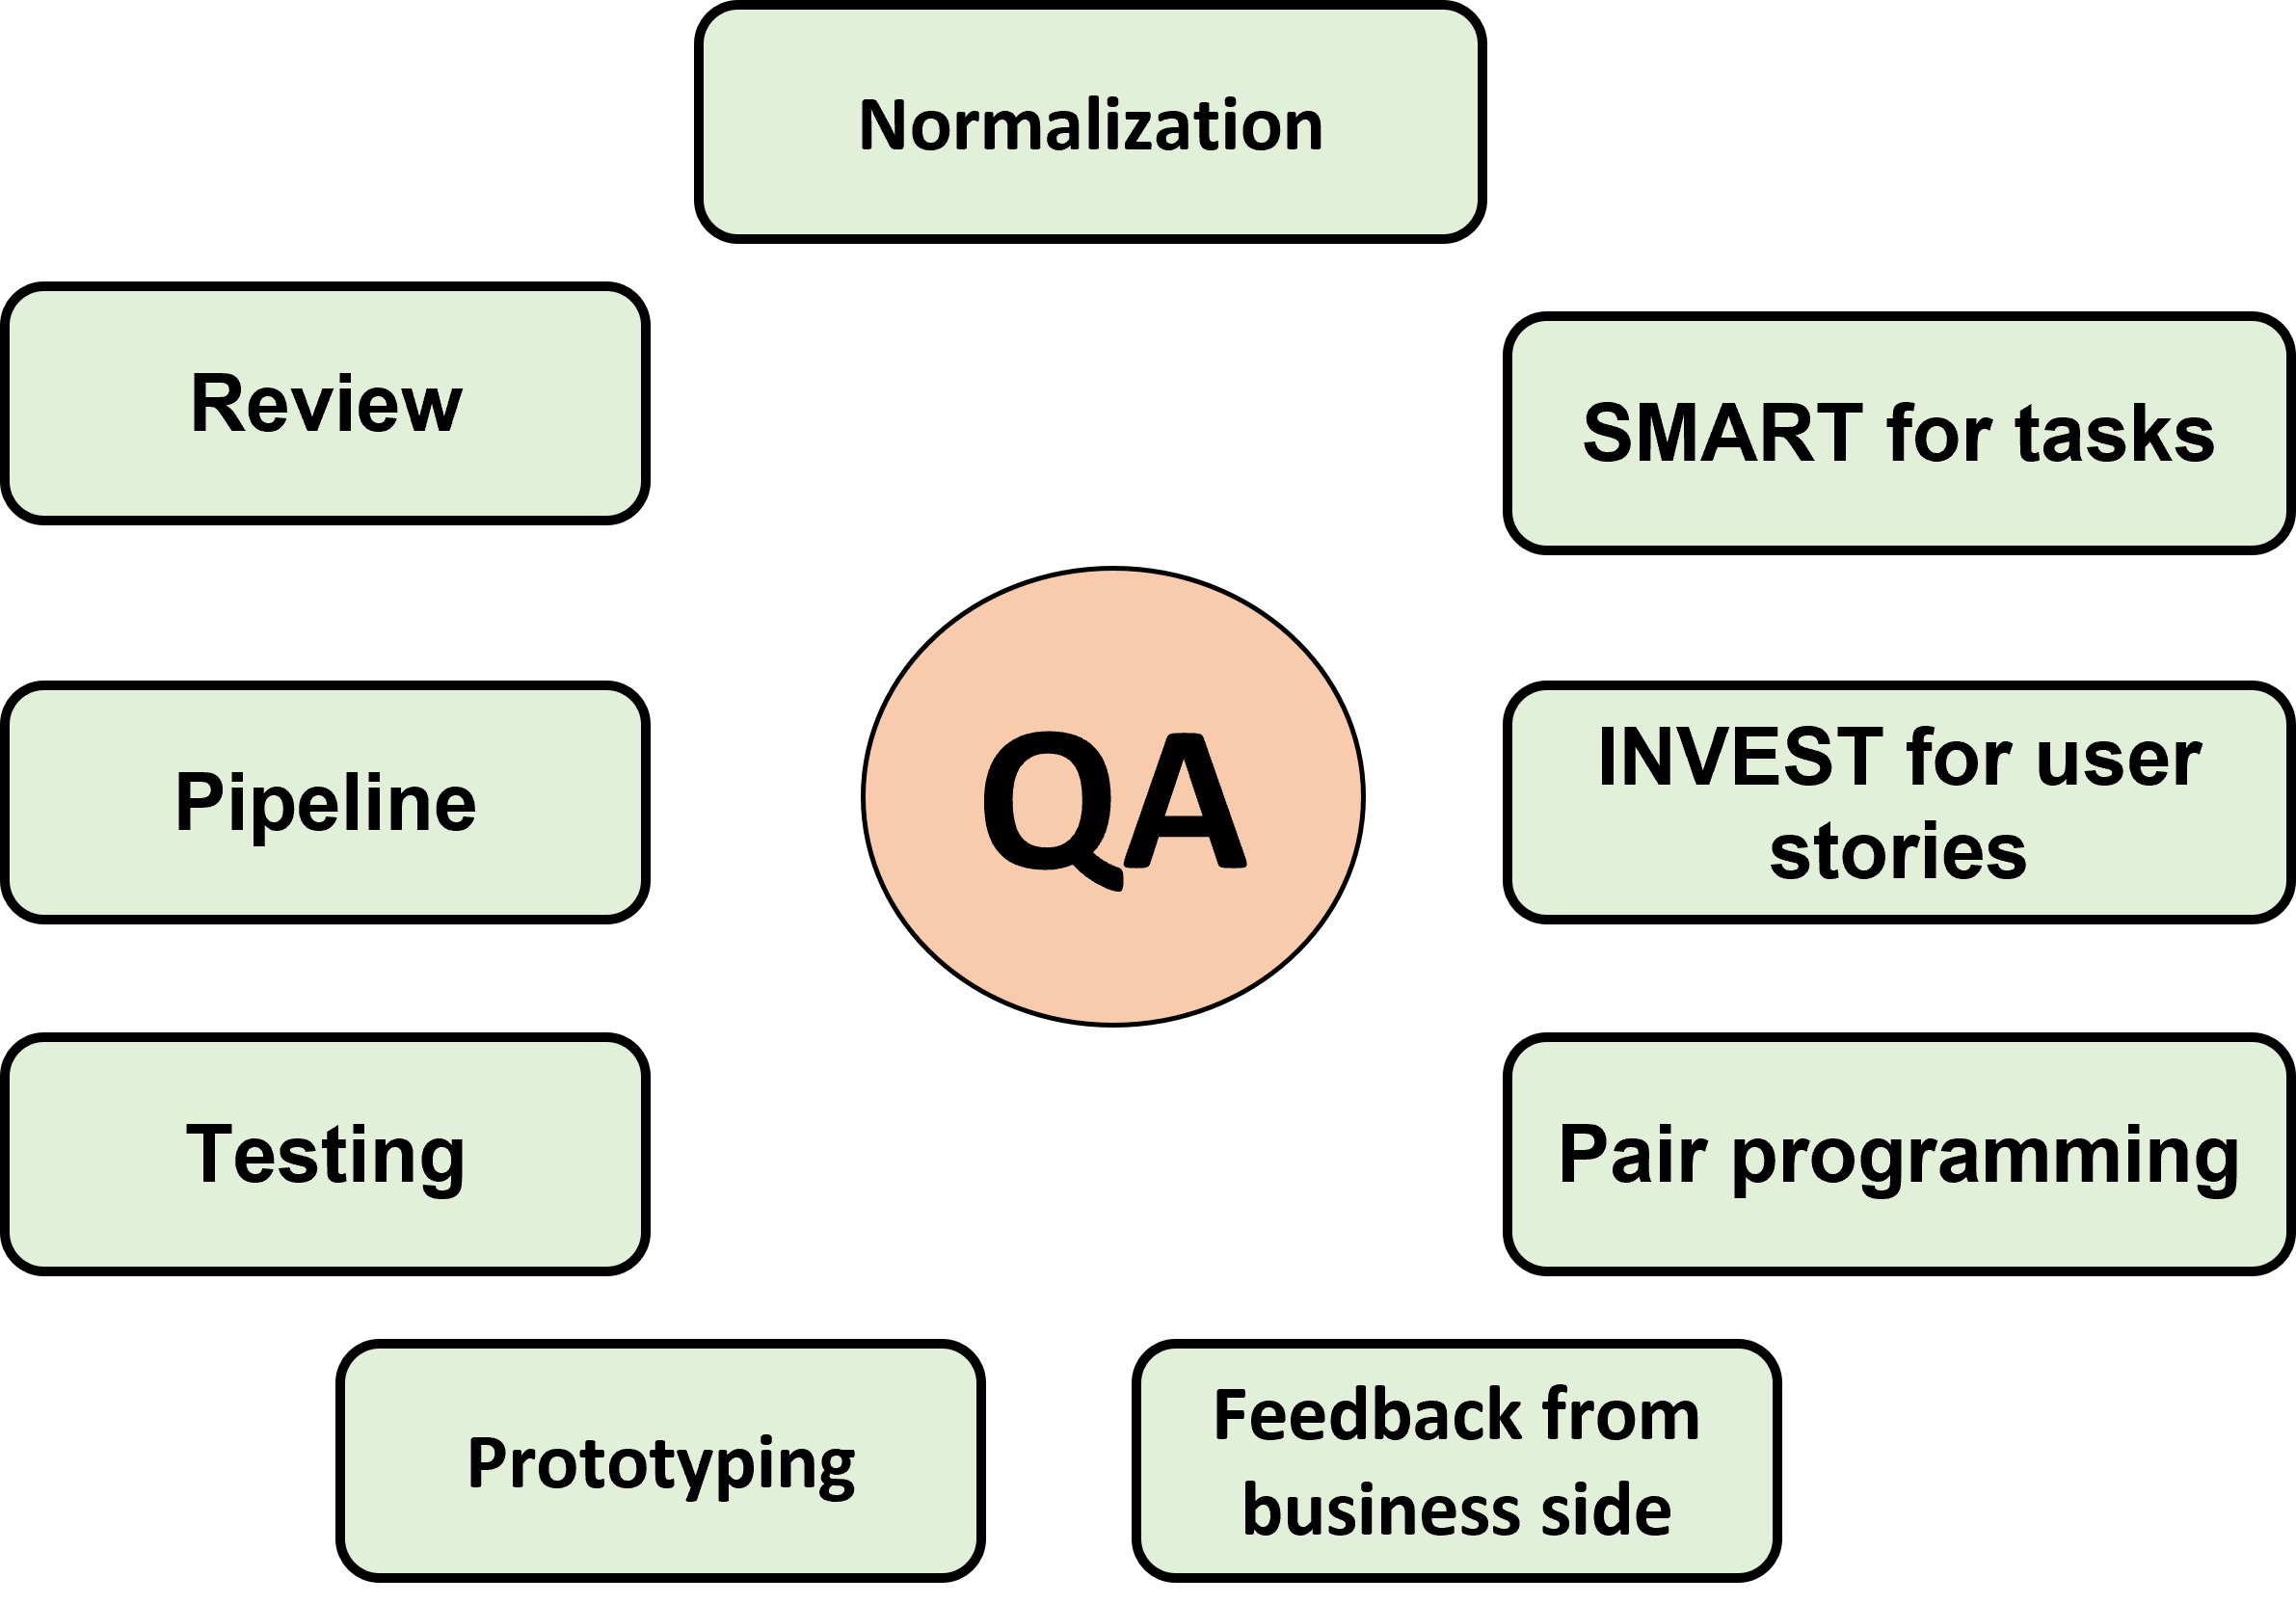
\includegraphics[scale=0.75]{resources/images/qa-techniques.png}
    \caption{QA techniques}
    \label{fig:qa-techniques}
\end{figure}